\documentclass[twoside]{article}
\usepackage[utf8]{inputenc}
\usepackage[]{fontenc}
\usepackage{graphicx}

\usepackage{anysize}
\marginsize{3cm}{3cm}{1cm}{3cm}

\title{Populációdinamika}
\date{\today}
\author{Kovács Kristóf Péter}

\begin{document}
	
	\maketitle
	\thispagestyle{empty}
	\begin{center}
		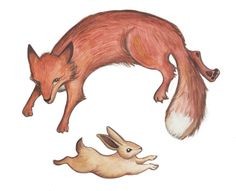
\includegraphics[width = 0.4\textwidth]{fox_n_rabbits}
		\\
		\tiny{Kép: Fox and Hare,
		\\hannahaha (devianart), 2011.}
	\end{center}
	\pagebreak
	\section*{A program}
		A program két állatcsoport, számának változásait mutatja be, egy ragadozókból állóét, és annak zsákmányáét. Nem differenciálegyenleteket használ, hanem minden állatot egyenként szimulál.
		\subsection*{Állatok szimulálása}
			Egy állat véletlenszerúen talál táplálékot, melyet egy faktor befolyásol (például a zsákmány száma). Ha nem talál semennyit, elpusztul. Ha egy bizonyos mennyiséghez hozzájut szaporodni fog.
			\par Egy jóllakott hím és nőstény állat a szaporulatnak megfelelő utódot hoz létre. A nemeket az állatok véletlenszerűen kapják.
			\par Az állatoknak van egy megadott élettartama is.
		\subsection*{Léptetés}
			Az állatokat két láncolt listában tároltam. Egy körben ezeken a listákon iterálnak végig ciklusok. A sorra kerülő állat élelmet keres, majd, ha eleget talált, egy szintén jóllakott párt.
			\par A párkeresés a már korábban táplálkozott állat közül történik. A párzás egyel csökkenti a két példány éhségét, így nem kerülnek többször kiválasztásra.
			\par Egy kör lejátszása emiatt a módszer miatt magas példányszám mellett igen hosszúra nyúlhat.
		
	\section*{Eremények}
		\par A program nagyon érzékeny volt a kezdeti feltételekre. Sokszor előfordult, hogy pár kör alatt kihalt egyik vagy másik faj, vagy a számuk fokozatosan nőtt, amíg a program túlzottan le nem lassult.
		\subsection*{Kapott adatok}	
		\par Az alábbi diagram egy fenntartható arányt mutat:
		\begin{center}
			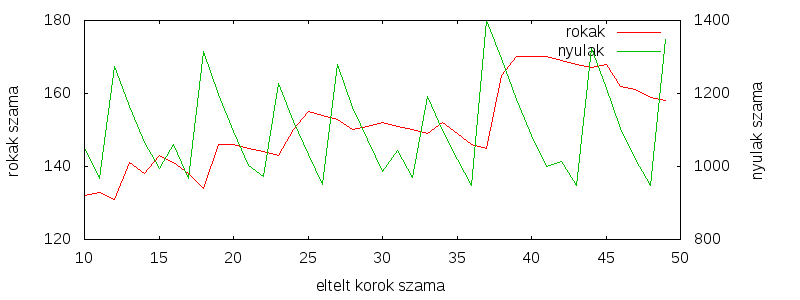
\includegraphics[width = \textwidth]{../build/eredmenyek.png}
		\end{center}
		\par Kezdeti feltételek:
		\begin{center}
			\begin{tabular}{crrc}
				&róka&nyúl&\\
				példányszám&10&100&\\
				élettartam&7&3&\\
				napi élelem&2&(1)&\\
				&&&\\
				\multicolumn{4}{l}{a rókák 11--szer annyi nyúl mellett vadásznak 100\%-os sikerrel}\\
			\end{tabular}
		\end{center}
		\par Megfigyelhető, hogy a nyulak száma mindig 1000 köré esik vissza, ennek oka, hogy a rókák itt nem tudták szabályozni a nyulak számát, e miatt be kellett vezetni a nyulaknak is egy táplálékforrást, ami 1000 nyulat tud megfelelően eltartani. Az arány közel ugyanaz maradt, mint kezdetben, azaz 11-szeres.
		\par Ezt azt jelzi, hogy mérvadóan csak a táplálékforrás szabályozta az populációt.
		
	\pagebreak
	\section*{A projekt}
	\subsection*{Létrehozás}
		A projekt a \textbf{cmake} segítségével jön létre. A C++ és \LaTeX\ fájlok fordítását, valamint az adatok Gnuplottal történő ábrázolását CMakeList.txt-k vezérlik.\par 
		A projekt legfelső szintjén csak az almappák vannak megadva. Az összetevők négy almappába vannak rendezve: kettő a programnak (futtatható és egyéb programrészek), egy a plottolásnak és egy az ezen dokumantum létrehozásához szükséges forrásoknak.\par 
		Három target szerepel a makefile-okban. Mindegyiknek feltétele az előtte levő megléte, tehát, ha üresen indítjuk el a dokumentumot, lefordulnak a forrásfájlok is, stb...\par 
		\subsubsection*{szim\_futtatas}
		Gyakorlatilag a program lefordítása és futtatása. A program által kiadott adatsortól függ, amely annak a \textbf{custom\_command}-nak a kimenete, amely a programrészek lefordítását és összelinkelését vezérlő alprojektet indítja el.\par 
		\subsubsection*{plottolas}
		A kiadott adatsort ábrázolja a Gnuplot programmal, az elkészült png fáljtól függ. Az ezt létrehozó custom\_command a konzolon is beírható \par
		{ \centering \textgreater\ gnuplot script.p \par }
		parancsot hajtja végre. Szükséges hozzá még a Gnuplot package.
		\subsubsection*{dokumentum}
		A végső PDF létrehozásáért felel. Egy kiegészítő cmake fájlt haszál fel, amit a mappája tartalmaz is. A latex fordító igen érzékeny a képek helyének hivatkozásaira, ezért a használt \textbf{UseLATEX.cmake} minden képet lemásol és megfelelő útvonalat alkotó mappákba rakja őket. A még nem plottolt ábrákkal ezt nem tudná megtenni, ezért helyettük felülírhatő cserefájlokat generál.\par 
	\subsection*{Megosztás}
		A programot és annak változásait a saját gépemen a \textbf{git} segítségével mentettem el a \textit{git add .} és \textit{git commit} parancsokkal a helyi repository-ba. \par
		A kész mentéseket a \textit{git push} paranccsal töltöttem fel a korábban elkészített online repository-ba, előtte beállítva annak url-jét a \textit{git remote add} paranccsal.
\end{document}
